\documentclass[10pt]{beamer}
\usetheme[
%%% option passed to the outer theme
%    progressstyle=fixedCircCnt,   % fixedCircCnt, movingCircCnt (moving is deault)
  ]{Feather}
  
% If you want to change the colors of the various elements in the theme, edit and uncomment the following lines

% Change the bar colors:
%\setbeamercolor{Feather}{fg=red!20,bg=red}

% Change the color of the structural elements:
%\setbeamercolor{structure}{fg=red}

% Change the frame title text color:
%\setbeamercolor{frametitle}{fg=blue}

% Change the normal text color background:
%\setbeamercolor{normal text}{fg=black,bg=gray!10}

%-------------------------------------------------------
% INCLUDE PACKAGES
%-------------------------------------------------------

\usepackage[utf8]{inputenc}
\usepackage[english]{babel}
\usepackage[T1]{fontenc}
\usepackage{helvet}

%-------------------------------------------------------
% DEFFINING AND REDEFINING COMMANDS
%-------------------------------------------------------

% colored hyperlinks
\newcommand{\chref}[2]{
  \href{#1}{{\usebeamercolor[bg]{Feather}#2}}
}

%-------------------------------------------------------
% INFORMATION IN THE TITLE PAGE
%-------------------------------------------------------

\title[Analizadores de proceso]{ }
\author{Mauricio Ordoñez Prieto}
\institute{Universidad Distrital Francisco Jose de Caladas}
\date{24 de Septiembre de 2017}

%-------------------------------------------------------
% THE BODY OF THE PRESENTATION
%-------------------------------------------------------

\begin{document}

%-------------------------------------------------------
% THE TITLEPAGE
%-------------------------------------------------------

{\1% % this is the name of the PDF file for the background
\begin{frame}{Analizadores de proceso}{ }
Es todo el conjunto de ideas, tecnología, diseño, instrumentos, equipos o servicios que bien seleccionados y ordenadamente relacionados entre sí, contribuyen a obtener resultados analíticos fiables.
\begin{figure}%%Inicia paquete para cargar figura
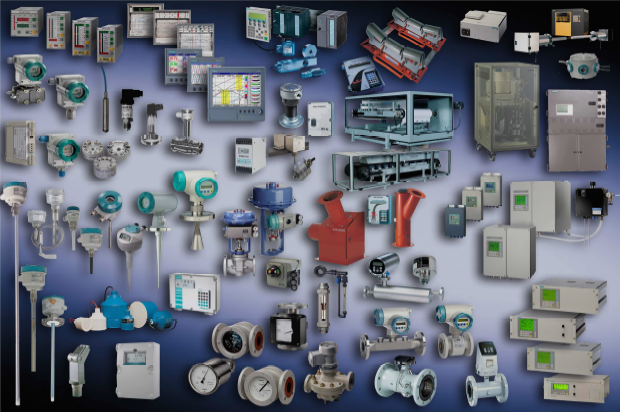
\includegraphics[width=0.5\textwidth]{figura_4.png} %%Escala figura y la llama
\caption{\label{fig:1}Analizadores de Proceso} %% Nombre de la figura y pone una etiqueta 
\end{figure}
\end{frame}
\begin{frame}{Analizadores de Proceso}{ }  
\begin{center}
\end{center}
\vskip 0.5cm
\begin{center}
En los procesos industriales, según la severidad de las especificaciones se han desarrollado diferentes estrategias de control que requieren conocimiento puntual de ciertas variables que determinan la calidad del proceso.
\end{center}
\end{frame}
%-------------------------------------------------------%%%
%-------------------------------------------------------
%-------------------------------------------------------
\begin{frame}{Variables en procesos industriales}{}
\begin{block}{}
  \begin{itemize}
    \item {\tt Presión}
    \item {\tt Temperatura}
    \item {\tt Caudal}
    \item {\tt Nivel}
    \item {\tt Posicionamiento}
    \item {\tt Protección}
    \item {\tt Reguladores}
    \item {\tt Pesaje Estático}
    \item {\tt Pesaje Dinámico}
    \item {\tt Analizado de Gases}
    \item {\tt Cromatógrafos}
    \item {\tt Espectrometro}
    \item {\tt Analizador de Líquidos}
  	\end{itemize}
	\end{block}
	\end{frame}
	\begin{frame}{¿Para que sirve un analizador de proceso?}{}
Los analizadores de procesos modernos permiten evaluar la calidad de las medidas analíticas que comprende un proceso determinado.
\begin{figure}%%Inicia paquete para cargar figura
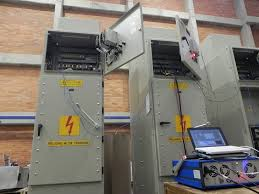
\includegraphics[width=0.5\textwidth]{figura_3.jpg} %%Escala figura y la llama
\caption{\label{fig:2}Analizador Eléctrico} %% Nombre de la figura y pone una etiqueta 
\end{figure}
\end{frame}
%-------------------------------------------------------
\begin{frame}{Clasificación de analizadores de proceso}{}
De acuerdo a su aplicación y a sus características esenciales, se clasifican en cinco grandes grupos.  
\begin{block}{ }
Analizadores de proceso:
  \begin{itemize}
    \item {\tt Analizadores de Técnicas Generales: Cromatografía, absorción, infrarojos, entre otros.}
    \item {\tt Analizadores de propiedades físicas}
    \item {\tt Aplicaciones Especificas:Determinada calidad o componente}
    \item {\tt Análisis de Gases}
    \item {\tt Analizadores en control de calidad de aguas}
  	\end{itemize}
	\end{block}
\end{frame}
%%%%%%%%%%%%
\begin{frame}{Clases de analizadores}{ }
\begin{block}{ }
Clases de analizadores de proceso:
  	\begin{itemize}
    \item {\tt In-Situ o Extractivos}
    \item {\tt Para Líquidos y Gases}
    \item {\tt Propiedades Físicas}
    \item {\tt Continuos o Cíclicos}
    \item {\tt Composición}
    \item {\tt Calidad de aire-emisiones,inmisiones}
    \item {\tt Calidad de Agua}
    \item {\tt Química Húmeda}
    \item {\tt Aplicación y uso}
    \item {\tt Control de procesos}
  	\end{itemize}
	\end{block}
    \end{frame}
%-------------------------------------------------------

%-------------------------------------------------------


%-------------------------------------------------------
\begin{frame}{In-Situ o Extractivos}{Clases de analizadores de proceso}
Son analizadores que se encuentran montados y midiendo directamente sobre el proceso, analizadores In -Situ y analizadores montados fuera de este y que analizan una muestra que es extraída de la corriente del proceso determinado. 
\begin{figure}%%Inicia paquete para cargar figura
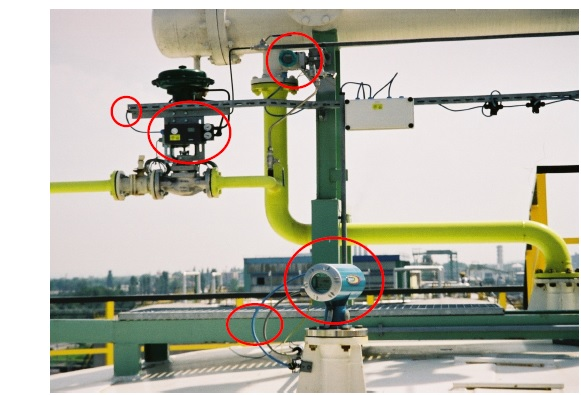
\includegraphics[width=0.5\textwidth]{figura_7.jpg} %%Escala figura y la llama
\caption{\label{fig:3}Analizadores de Proceso In-Situ} %% Nombre de la figura y pone una etiqueta 
\end{figure}
\end{frame}

%-------------------------------------------------------
\begin{frame}{Para Líquidos o Gases}{Clases de analizadores de proceso}
analizadores de proceso In-Situ o extractivos son muy usados en la industria para determinar calidades y composición de fluidos. El tipo de muestra o medio a medir determina su clasificación. 
\begin{figure}%%Inicia paquete para cargar figura
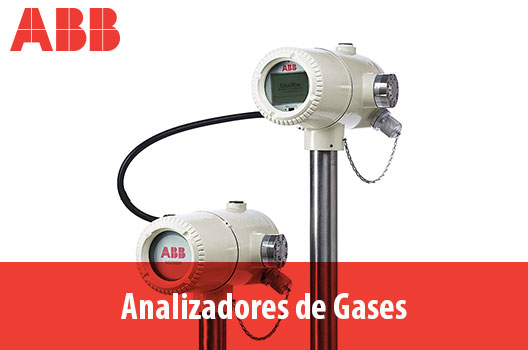
\includegraphics[width=0.3\textwidth]{figura_8.jpg} %%Escala figura y la llama
\caption{\label{fig:4}Analizadores de gases} %% Nombre de la figura y pone una etiqueta 
\end{figure}
\begin{figure}%%Inicia paquete para cargar figura
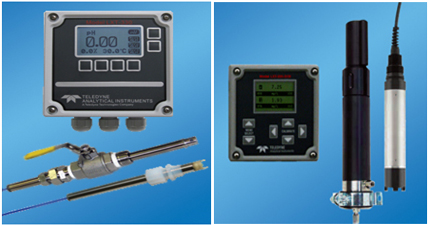
\includegraphics[width=0.3\textwidth]{figura_9.jpg} %%Escala figura y la llama
\caption{\label{fig:5}Analizadores de Líquidos} %% Nombre de la figura y pone una etiqueta 
\end{figure}
\end{frame}
%-------------------------------------------------------   
  \begin{frame}{Propiedades Físicas}{Clases de analizadores de proceso}
Son aquellos utilizados en la industria para medir cierto valor de una propiedad física de las cuales podemos mencionar:
Analizadores para Viscosidad, analizadores para densidad, punto de destilación, punto de congelación y punto de cristalización. 
\begin{figure}%%Inicia paquete para cargar figura
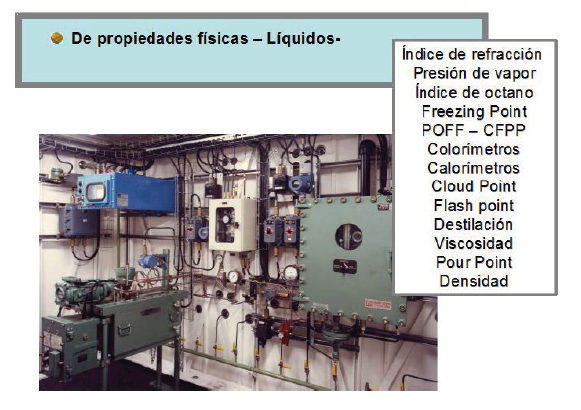
\includegraphics[width=0.5\textwidth]{figura_10.png} %%Escala figura y la llama
\caption{\label{fig:6}Analizadores de propiedades físicas} %% Nombre de la figura y pone una etiqueta 
\end{figure}
\end{frame}  
%%%%%%%%%%%%%%%%%%%%%%%%%%%%%%%
%%%%%%%%%%%%%%%%%%%%%%%%%%%%%%%%
  \begin{frame}{Continuos o Cíclicos}{Clases de analizadores de proceso}
Los analizadores cíclicos realizan una secuencia determinada de análisis, al final del cual proporcionan o refrescan el resultado de la medida analítica.      
\begin{figure}%%Inicia paquete para cargar figura
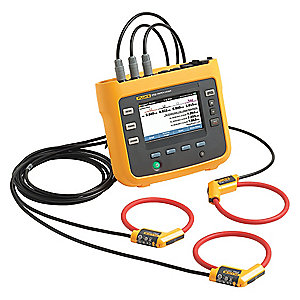
\includegraphics[width=0.4\textwidth]{figura_11.jpg} %%Escala figura y la llama
\caption{\label{fig:7}Analizador Eléctrico} %% Nombre de la figura y pone una etiqueta 
\end{figure}
\end{frame}  
 \begin{frame}{Composición}{Clases de analizadores de proceso}
Así se denominan aquellos instrumentos usados para medir la concentración de uno o varios determinados componentes dentro de una mezcla (Líquida o Gaseosa).     
\begin{figure}%%Inicia paquete para cargar figura
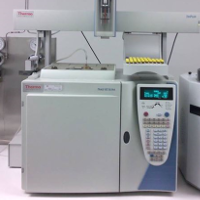
\includegraphics[width=0.1\textwidth]{figura_12.png} %%Escala figura y la llama
\caption{\label{fig:8}Cromatógrafo} %% Nombre de la figura y pone una etiqueta 
\end{figure}
\begin{figure}%%Inicia paquete para cargar figura
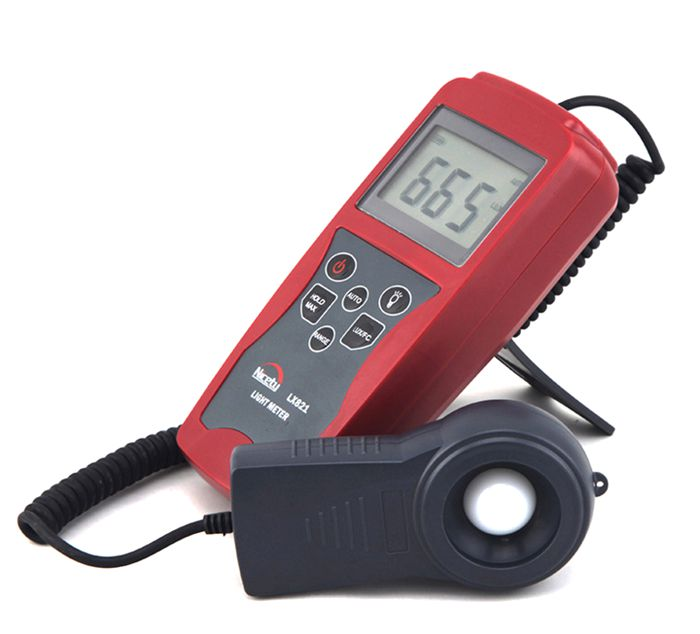
\includegraphics[width=0.1\textwidth]{figura_13.jpg} %%Escala figura y la llama
\caption{\label{fig:9}Fotómetro} %% Nombre de la figura y pone una etiqueta 
\end{figure}
\begin{figure}%%Inicia paquete para cargar figura
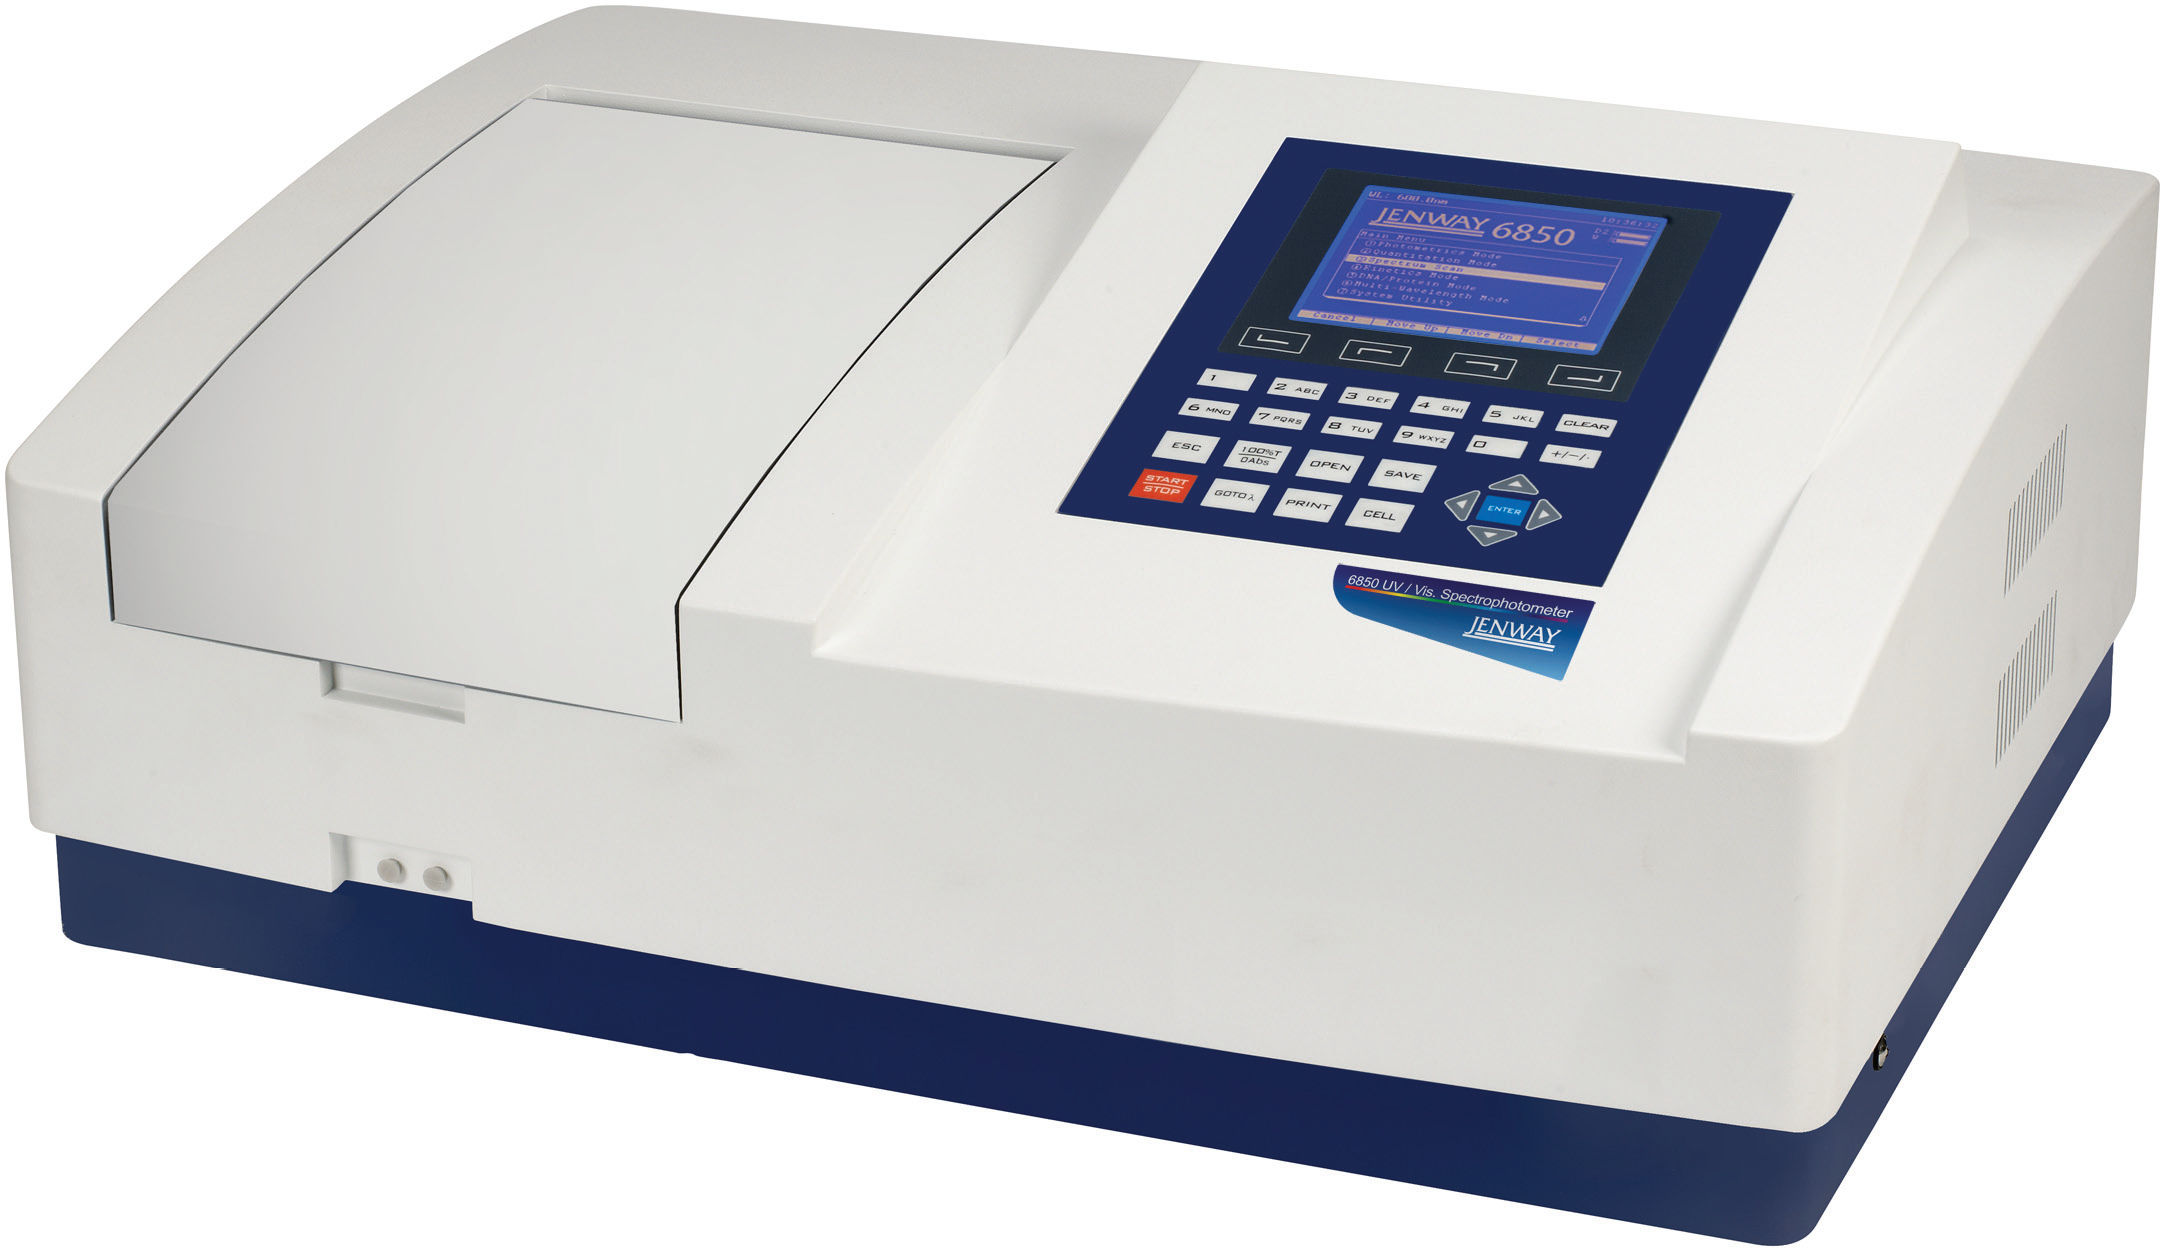
\includegraphics[width=0.1\textwidth]{figura_14.jpg} %%Escala figura y la llama
\caption{\label{fig:10}Espectometro} %% Nombre de la figura y pone una etiqueta 
\end{figure}
\end{frame}  
\begin{frame}{Calidad de Aire}{Clases de analizadores de proceso}
La protección del medio ambiente ha llevado a las distintas formas de legislar normas orientadas para mejorar la calidad del aire.
\vskip 0.5cm
Emisiones: para garantizar las cantidades máximas de contaminantes que se vierten, se exige a la industria que mida ciertos compuestos en los gases de combustión de calderas, generadores, incineradoras tanto industriales como municipales.
\begin{figure}%%Inicia paquete para cargar figura
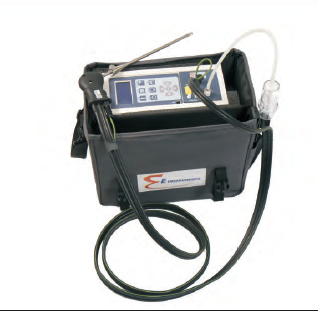
\includegraphics[width=0.3\textwidth]{figura_15.png} %%Escala figura y la llama
\caption{\label{fig:11}Analizador de emisiones de gases de combustión} %% Nombre de la figura y pone una etiqueta 
\end{figure}
\end{frame} 
\begin{frame}{Calidad de Aire}{Clases de analizadores de proceso}
Inmisiones: También se determina la concentración máxima de ciertos compuestos nocivos en el aire y que deben ser medidos de forma puntual o continua.
\begin{figure}%%Inicia paquete para cargar figura
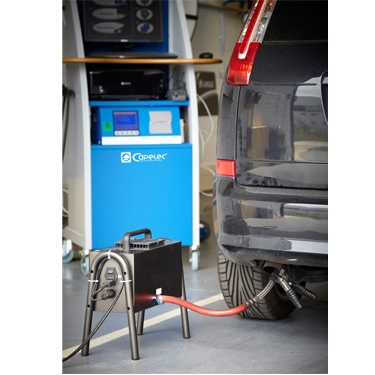
\includegraphics[width=0.3\textwidth]{figura_16.jpg} %%Escala figura y la llama
\caption{\label{fig:12}Analizador de emisiones de gases de combustión} %% Nombre de la figura y pone una etiqueta 
\end{figure}
\end{frame}   
%%%%%%%%%%%%%%%%%%%%%%%%%%%%%%%%%%%%%%%%%%%%%%%%%%%%%%%%%%%%%%%%%%%%%%%%%%%%%%%%%%%%%%%%%%%%%%%%%%%%%%%%%%%%%%%%%%%%%%
 
\begin{frame}{Calidad del Agua}{Clases de analizadores de proceso}
Otra línea importante de analizadores es la relativa a la medición de ciertas características físicas del agua, como el PH,la turbidez, la conductividad o la concentración de ciertos compuestos disueltos, como cloro, carbono orgánico, entre otros. 
\begin{figure}%%Inicia paquete para cargar figura
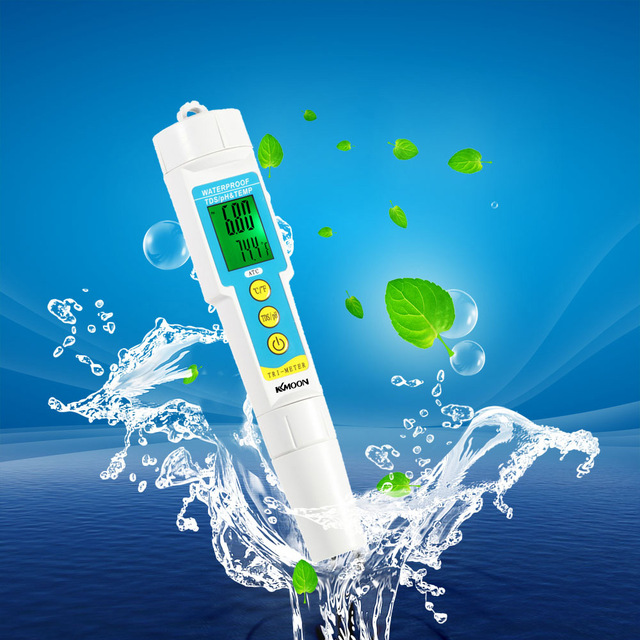
\includegraphics[width=0.3\textwidth]{figura_17.jpg} %%Escala figura y la llama
\caption{\label{fig:13}Analizador de calidad de agua} %% Nombre de la figura y pone una etiqueta 
\end{figure}
\end{frame}
%%%%%%%%%%%%%%%%%%%%%%%%%%%%%%%%%%%%%%%%%%%%%%%%%%%%%%%%%%%%%%%%%%%%%%%%%%%%%%%%%%%%%%%%%%%%%%%%%%%%%%%%%%%%%%%%%%%%%%%%%%%%%
\begin{frame}{Química Húmeda}{Clases de analizadores de proceso}
Son aquellos analizadores que realizan, de forma automatizada, una secuencia o método de análisis derivado de un procedimiento de laboratorio 
\begin{figure}%%Inicia paquete para cargar figura
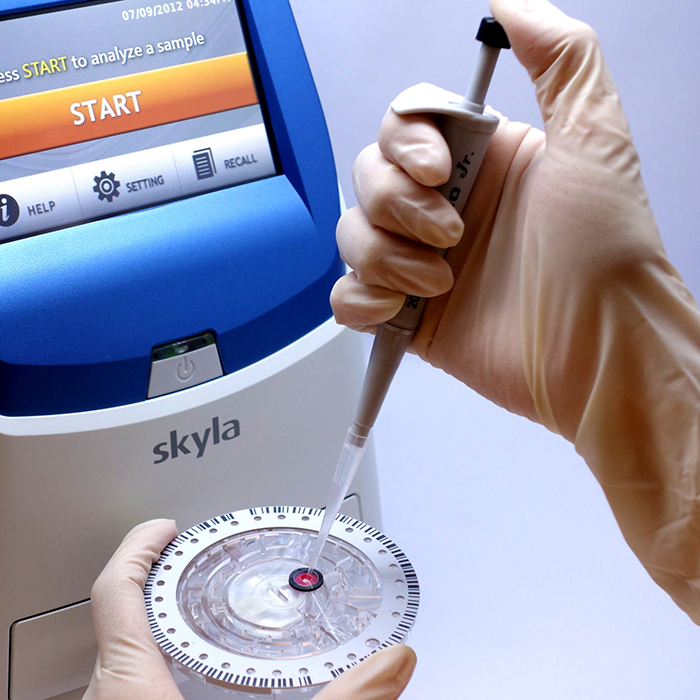
\includegraphics[width=0.3\textwidth]{figura_18.jpg} %%Escala figura y la llama
\caption{\label{fig:14}Analizador automático de bioquímica} %% Nombre de la figura y pone una etiqueta 
\end{figure}
\end{frame}
 %%%%%%%%%%%%%%%%%%%%%%%%%%%%%%%%%%%%%%%%%%%%%%%%%%%%%%%%%%%%%%%%%%%%%%%%%%%%%%%%%%%%%%%%%%%%%%%%%%%%%%%%%%%%%%%%%%%%%%%%%%%%%%%%%%
 \begin{frame}{Por su Aplicación o Uso }{Clases de analizadores de proceso}
 Otra forma de clasificar a los analizadores de proceso de basa en la aplicación de cada analizador o el uso que se le da a la medida analítica. 
\begin{block}{ }
Se pueden emplear en:
  	\begin{itemize}
    \item {\tt Control de Procesos}
    \item {\tt Control de Calidad}
    \item {\tt Identificación Positiva}
    \item {\tt Medio Ambiente}
    \item {\tt Seguridad}
    \end{itemize}
	\end{block}
 	\vskip 0.5cm
Cuando el analizador se usa en control de procesos significa que forma parte de un determinado lazo de control en alguno de los diferentes niveles de control.
\end{frame}
 %%%%%%%%%%%%%%%%%%%%%%%%%%%%%%%%%%%%%%%%%%%%%%%%%%%%%%%%%%%%%%%%%%%%%%%%%%%%%%%%%%%%%%%%%%%%%%%%%%%%%%%%%%%%%%%%%%%%%%%%%%%%%%%%%%%
 \begin{frame}{Niveles de Control}{Analizadores de proceso}
 En la actualidad, con los ordenadores y los sistemas digitales de control se consideran, básicamente tres niveles de control, cada uno de los cuales tiene sus requerimientos específicos para los analizadores de proceso.
 \begin{figure}%%Inicia paquete para cargar figura

\includegraphics[width=0.5\textwidth]{figura_19.jpg} %%Escala figura y la llama
\caption{\label{fig:15}niveles de control} %% Nombre de la figura y pone una etiqueta 
\end{figure}
\end{frame}
 
 %%%%%%%%%%%%%%%%%%%%%%%%%%%%%%%%%%%%%%%%%%%%%%%%%%%%%%%%%%%%%%%%%%%%%%%%%%%%%%%%%%%%%%%%%%%%%%%%%%%%%%%%%%%%%%%%%%%%%%%%%%%%%%%%%%%%%
  \begin{frame}{Nivel 1, Regulación}{Analizadores de proceso}
 Es el nivel en el que se desarrolla un control básico y directo del proceso.Ejemplo: sensores, transmisores, controladores, válvulas de control, entre otros.
 Los dos más importantes son:

 \begin{block}{ }
 Los requisitos más importantes son:
  	\begin{itemize}
    \item {\tt Respuesta rápida}
    \item {\tt Fiabilidad}
    \end{itemize}
	\end{block}
    \end{frame}
 
 %%%%%%%%%%%%%%%%%%%%%%%%%%%%%%%%%%%%%%%%%%%%%%%%%%%%%%%%%%%%%%%%%%%%%%%%%%%%%%%%%%%%%%%%%%%%%%%%%%%%%%%%%%%%%%%%%%%%%%%%%%%%%%%%%%
   \begin{frame}{Nivel 2, Control Supervisorio}{Analizadores de proceso}
Normalmente se realiza por medio de un  sistema de control de proceso, generalmente con un sistema de instrumentación digital.
\vskip 0.5cm
La señal del analizador se suele usar como punto de consigna del controlador principal.
\end{frame}
%%%%%%%%%%%%%%%%%%%%%%%%%%%%%%%%%%%%%%%%%%%%%%%%%%%%%%%%%%%%%%%%%%%%%%%%%%%%%%%%%%%%%%%%%%%%%%%%%%%%%%%%%%%%%%%%%%%%%%%%%%%%%%%%%%%%%%%%%
 \begin{frame}{Nivel 3, Control de Optimización}{Analizadores de proceso}
Se lleva a cabo en el sistema de control de proceso a un nivel más elevado dado que en los cálculos y algoritmos de optimización entran ciertos factores 
económicos como:rentabilidad, oferta y demanda, costos, materias primas, entre otros.   
\vskip 0.5cm
A este nivel de control, el tiempo de respuesta puede ser bastante lento, de forma que hay una gran campo de aplicaciones de los analizadores de proceso.
\end{frame}
%%%%%%%%%%%%%%%%%%%%%%%%%%%%%%%%%%%%%%%%%%%%%%%%%%%%%%%%%%%%%%%%%%%%%%%%%%%%%%%%%%%%%%%%%%%%%%%%%%%%%%%%%%%%%%%%%%%%%%%%%%%%%%%%%%%%%%%%%%%%%%%%%%%%%%%%%%%%%%%%%%%%%%%%%%%%%%%%%%%%%%%%%%%%%%%%%%%%%%%%%%%%%%%%%%%%%%%%%%%%%%%%
 \begin{frame}{Algunos Criterios en control}{Analizadores de proceso}
Existen dos factores importantes que se deben considerar cuando se usen analizadores en control de procesos.
 \begin{block}{ }
  	\begin{itemize}
    \item {\tt Tiempo de respuesta del sistema}
    \item {\tt Fiabilidad y factor de servicio del sistema analítico}
    \end{itemize}
	\end{block}
    \end{frame}
 %%%%%%%%%%%%%%%%%%%%%%%%%%%%%%%%%%%%%%%%%%%%%%%%%%%%%%%%%%%%%%%%%%%%%%%%%%%%%%%%%%%%%%%%%%%%%%%%%%%%%%%%%%%%%%%%%%%%%%%%%%%%%%%%%
 \begin{frame}{Algunos Criterios en control}{Analizadores de proceso}
El tiempo de respuesta depende en gran medida del sistema de muestra.
\vskip 0.5cm
La fiabilidad y el factor de servicio vienen determinados por la calidad del propio analizador, el diseño del sistema, su instalación y la cantidad de su mantenimiento, así como del método y frecuencia de calibración.   
\end{frame}
%%%%%%%%%%%%%%%%%%%%%%%%%%%%%%%%%%%%%%%%%%%%%%%%%%%%%%%%%%%%%%%%%%%%%%%%%%%%%%%%%%%%%%%%%%%%%%%%%%%%%%%%%%%%%%%%%%%%%%%%%%%%%%%%%%%%%%%%%%%%%%%%%%%%%%%%%%%%%%%%%%%%%%%%%%%%%%%%%%%%%%%%%%%%%%%%%%%%%%%%%
\begin{frame}{Parametros esenciales}{Analizadores de proceso}
Para cualquier tipo de analizador hay una serie de parametros que permiten determinar la calidad de sus medidas.
\begin{block}{ }
Estos parámetros son:
  	\begin{itemize}
    \item {\tt Exactitud}
    \item {\tt Precisión o repetibilidad}
    \item {\tt Reproducibilidad}
    \item {\tt Sensibilidad}
    \item {\tt Linealidad}
    \item {\tt Ruido}
    \item {\tt Tiempo de respuesta}
    \item {\tt Tiempo de ciclo }
    \item {\tt Deriva de cero}
    \item {\tt Deriva de Span}
    \end{itemize}
	\end{block}  
\end{frame}
%%%%%%%%%%%%%%%%%%%%%%%%%%%%%%%%%%%%%%%%%%%%%%%%%%%%%%%%%%%%%%%%%%%%%%%%%%%%%%%%%%%%%%%%%%%%%%%%%%%%%%%%%%%%%%%%%%%%%%%%%%%%%%%%%%%%%%%%%%%%%%%%%%%%%%%%%%%%%%%%%%%%%%%%%%%%%%%%%%%%%%%%%%%%%%%%%%%%%%%

\begin{frame}{Normas Elementales }{Analizadores de proceso}
En el diseño detallado de cualquier proyecto se deben tener en cuenta una serie de normas elementales, ademas de las especificaciones y documentación generada durante la etapa inicial
del proyecto, el equipo de ingeniería debe de disponer del respaldo de las normas citadas a continuación.
\begin{block}{ }

  	\begin{itemize}
    \item {\tt EEMUA Desing and installations of On-line Analyser Systems}
    \item {\tt EEMUA Code of parctice for callibration and checking Process Analysers }
    \item {\tt IEC 79-16 Electrical apparatus for explosive atmospheres}
    \item {\tt NFPA 70.National electrical code,NEC }
    \item {\tt NFPA 496. Purged and pressurized enclosures for electrical equipment  }
    \end{itemize}
	\end{block}  
\end{frame}
%%%%%%%%%%%%%%%%%%%%%%%%%%%%%%%%%%%%%%%%%%%%%%%%%%%%%%%%%%%%%%%%%%%%%%%%%%%%%%%%%%%%%%%%%%%%%%%%%%%%%%%%%%%%%%%%%%%%%%%%%%%%%%%%%%%%%%%%%%%%%%%%%%%%%%%%%%%%%%%%%%%%%%%%%%%%%%%%%%%%%%%%%%%%%%%%%%%%%%%%%%%%%%%%%%%
\begin{frame}{Normas Elementales }{Analizadores de proceso}
\begin{block}{ }
  	\begin{itemize}
 	 \item {\tt UNE-EN 60079 para zonas clasificadas }
    \item {\tt  IEC 1285 Industrial proccess control }
    \item {\tt API 555 Process analyzers}
    \item {\tt Normas ASTM-IP relativas a métodos de análisis de propiedades físicas}
    \end{itemize}
	\end{block}  
\end{frame}

%%%%%%%%%%%%%%%%%%%%%%%%%%%%%%%%%%%%%%%%%%%%%%%%%%%%%%%%%%%%%%%%%%%%%%%%%%%%%%%%%%%%%%%%%%%%%%%%%%%%%%%%%%%%%%%%%%%%%%%%
 \begin{frame}{ Transmisor de presión}{Analizadores de proceso}

 \begin{figure}%%Inicia paquete para cargar figura
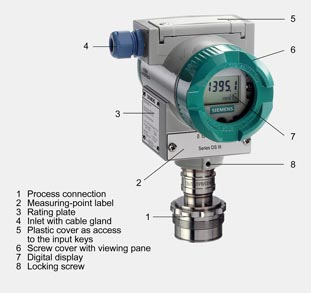
\includegraphics[width=0.6\textwidth]{figura_21.jpg} %%Escala figura y la llama
\caption{\label{fig:16} Trasmisor de presión Siemens } %% Nombre de la figura y pone una etiqueta 
\end{figure}
\end{frame}

%%%%%%%%%%%%%%%%%%%%%%%%%%%%%%%%%%%%%%%%%%%%%%%%%%%%%%%%%%%%%%%%%%%%%%%%%%%%%%%%%%%%%%%%%%%%%%%%%%%%%%%%%%%%%%%%%%%%%%%%%%%%%%%%%%%%%%%%

 \begin{frame}{ Transmisor de presión}{Analizadores de proceso}

 \begin{figure}%%Inicia paquete para cargar figura
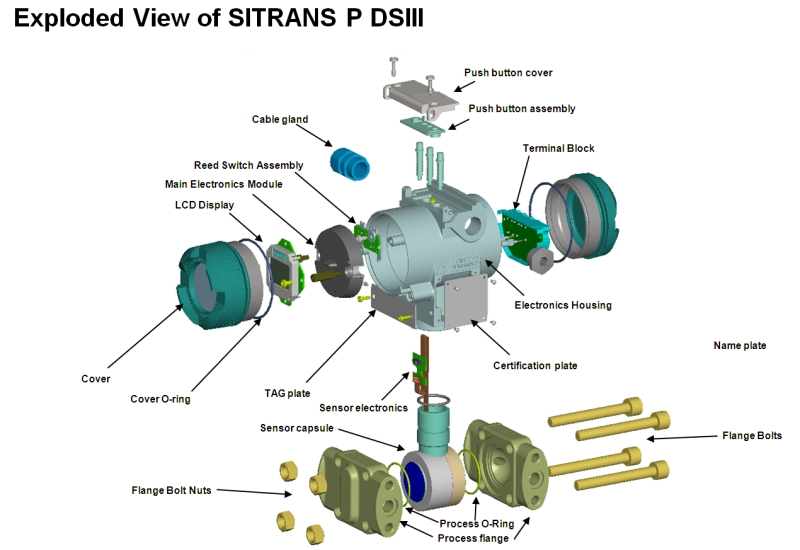
\includegraphics[width=0.7\textwidth]{figura_20.jpg} %%Escala figura y la llama
\caption{\label{fig:17} Trasmisor de presión Siemens } %% Nombre de la figura y pone una etiqueta 
\end{figure}
\end{frame}

%%%%%%%%%%%%%%%%%%%%%%%%%%%%%%%%%%%%%%%%%%%%%%%%%%%%%%%%%%%%%%%%%%%%%%%%%%%%%%%%%%%%%%%%%%%%%%%%%%%%%%%%%%%%%%%%%%%%%%%%%%%%%%%%%%%
 \begin{frame}{ Transmisor de presión}{Analizadores de proceso}
 \begin{figure}%%Inicia paquete para cargar figura
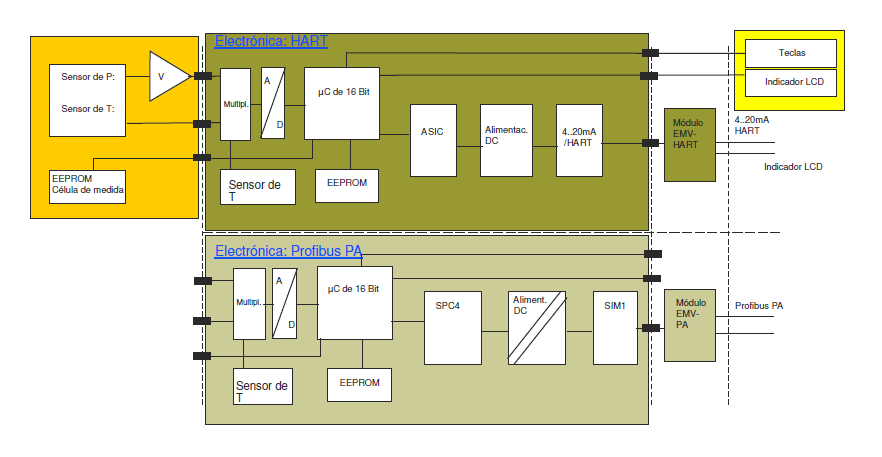
\includegraphics[width=0.9\textwidth]{figura_22.png} %%Escala figura y la llama
\caption{\label{fig:18} Trasmisor de presión Siemens } %% Nombre de la figura y pone una etiqueta 
	\end{figure}
	\end{frame}
%%%%%%%%%%%%%%%%%%%%%%%%%%%%%%%%%%%%%%%%%%%%%%%%%%%%%%%%%%%%%%%%%%%%%%%%%%%%%%%%%%%%%%%%%%%%%%%%%%%%%%%%%%%%%%%%%%%%%%%%%%%%%%%%%%%%%%%%%%%%%%%%%%%%%%%%%%%%%%%%%%%%%%%%%%%%%%%%%%%%%%%%%%%%%%%%%%%%%%%%%%%%%%%%%%%%%%%%%%%%%%%%%%%%%%%
 \begin{frame}{ Red profibus}{Analizadores de proceso}
 \begin{figure}%%Inicia paquete para cargar figura
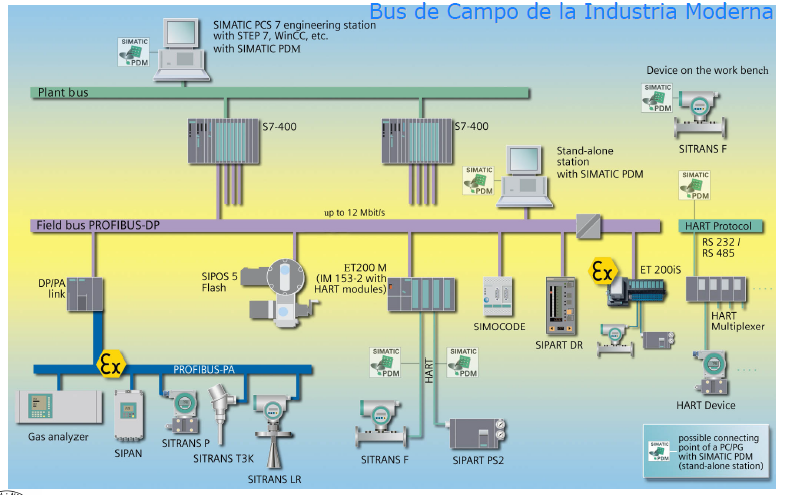
\includegraphics[width=0.9\textwidth]{figura_23.png} %%Escala figura y la llama
\caption{\label{fig:19} Red profibus} %% Nombre de la figura y pone una etiqueta 
	\end{figure}
	\end{frame}
%%%%%%%%%%%%%%%%%%%%%%%%%%%%%%%%%%%%%%%%%%%%%%%%%%%%%%%%%%%%%%%%%%%%%%%%%%%%%%%%%%%%%%%%%%%%%%%%%%%%%%%%%%%%%%%%%%%%%%%%%%%%%%%%%%%%%
\begin{frame}{Referencias}{Analizadores de proceso}
\begin{block}{ }
  	\begin{itemize}
    \item {\tt  Alfredo Rosado. Instrumentación de procesos:visión general y tecnologías de medición.
    Universidad de Valencia. }
    \item {\tt Francisco Velasco Aparicio. 2015. Analizadores de proceso en línea. España. }
    \item {\tt F.Velasco.2010.Analizadores de proceso, diseño de sistemas.}
    \end{itemize}
	\end{block}  
\end{frame}
%%%%%%%%%%%%%%%%%%%%%%%%%%%%%%%%%%%%%%%%%%%%%%%%%%%%%%%%%%%%%%%%%%%%%%%%%%%%%%%%%%%%%%%%%%%%%%%
{\1
\begin{frame}[plain,noframenumbering]
  \finalpage{¡Gracias por su Atención!}
\end{frame}}
\end{document}

%%%%%%%%%%%%%%%%%%%%%%%%%%%%%%%%%%%%%%%%%%%%%%%%%%%%%%%%%%%%%%%%%%%%%%%%%%%%%%%%%%%%%%%%%%%%%%%%%%%%%%%%%%%%%%%%%